\section{Extraction of Dynamic KG Summaries}
\label{sec:approaches-dynamic}

Dynamic summaries are extracted to tailor a KG to users' needs. Existing methods consider needs expressed in different manners: keyword queries, or personal interests.

\subsection{Query-Biased Summarization}

Snippet generation for KG search~\cite{DBLP:conf/cikm/ChenWCKQ19} and query-based KG exploration~\cite{DBLP:conf/cidr/LissandriniMHP22} can both be formulated as extracting a query-biased subgraph from a given KG. Early methods in this category solve it as a node/edge ranking problem. Recently, various formulations in combinatorial optimization have been adopted, in particular based on Group Steiner Trees for reflecting connections among query keywords in the graph structure. Not limited to maximizing the coverage of query keywords, they consider answer compactness and cohesiveness. Figure~\ref{fig:outline-gst} outlines the expressivity increases among different problem formulations.

\begin{figure}[h]
\centering
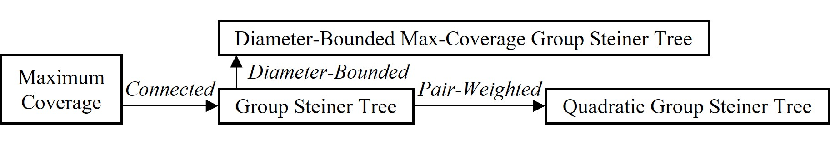
\includegraphics[width=\columnwidth]{figs/outline-gst.pdf}
\caption{Expressivity increases among problem formulations for query-biased extractive KG summarization.}
\label{fig:outline-gst}
\end{figure}

\subsubsection{Early Heuristics}
To acquaint the user with a KG in the context of keyword search, in an early work, Bai et al.~\shortcite{DBLP:conf/otm/BaiDT08} extract two subgraphs: a \emph{topic-oriented subgraph} for revealing the main topic of the KG, and a \emph{query-oriented subgraph} for showing its relevance to the query.
% which not only demonstrates the representative data samples of the given KG, but also matches the user's query intent.
The topic-oriented subgraph is extracted from the neighborhood of a topic entity based on predefined priorities of its properties; the topic entity is one that has a large indegree and outdegree. The query-oriented subgraph contain edges matched with query keywords; priority goes first to the edges incident with the topic entity.

\subsubsection{Maximum Coverage}
Instead of separately considering data representativeness and query relevance in two subgraphs, the KSD approach~\cite{DBLP:conf/semweb/WangCK19} jointly maximizes the coverage of all such elements of interest. Specifically, the elements of a KG that a summary is expected to cover include class and property instantiations, central entities, and keyword matches. To achieve it, a weighted \emph{Maximum Coverage} problem is formulated, where each edge (or type/attribute assertion) is represented as a set that may cover a class instantiation, a property instantiation, one or two entities, and/or a number of query keywords. Each class and property to be covered is weighted by its frequency in the KG. Each entity to be covered is assigned a weight measuring its graph centrality based on indegree and outdegree.
% Besides, each keyword is assigned an equal weight being inversely proportional to the total number of keywords in the query.
Solving this problem gives rise to a size-bounded optimum subgraph that maximizes the coverage of representative and query-biased data elements of the KG. As illustrated in Figure~\ref{fig:ksd}, the summary extracted by this approach is comparable with the summary extracted by IlluuSnip shown in Figure~\ref{fig:illusnip}. Given a keyword query \textit{Titanic US}, whereas both summaries include the most frequently instantiated class \texttt{Person} and property \texttt{act\_in} in Figure~\ref{fig:example}, the summary here further includes the entity \texttt{US} to match the query, although it is not required to be a connected subgraph.

\begin{figure}[h]
\centering
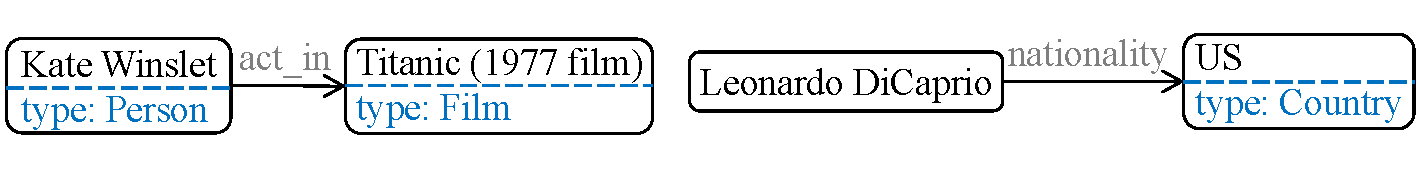
\includegraphics[width=\columnwidth]{figs/ksd.pdf}
\caption{A summary extracted from Figure~\ref{fig:example} containing the most frequently instantiated class \texttt{Person} and property \texttt{act\_in}, and containing the query keywords \textit{Titanic} and \textit{US}.}
\label{fig:ksd}
\end{figure}

\subsubsection{Group Steiner Tree}
Independent coverage of KG elements will easily produce a summary composed of multiple disconnected fragments. This weakens the structural cohesiveness of the summary, and misses the connections between keyword matches in the KG, which could be important to the user's judgment of query relevance. To overcome this limitation, a recent line of research formulates and solves a minimum-weight \emph{Group Steiner Tree} (GST) problem~\cite{DBLP:conf/wg/Ihler91}. The KeyKG approach~\cite{DBLP:conf/www/Shi0K20} maps each query keyword to a group of entities, and the target is a minimum-weight tree that covers all the groups, i.e., contains at least one matched entity for each keyword. Edge weights can be defined by an off-the-shelf method depending on the application. The resulting tree concisely reflects a structural relationship among all the query keywords. For example, given a keyword query \textit{Titanic US}, the summary in Figure~\ref{fig:gst} includes a path that connects the two query keywords. Considering the NP-hardness of this problem, KeyKG features a new approximation algorithm that employs an offline computed distance index to accelerate online extraction of shortest paths between groups to be merged into a tree.

\begin{figure}[h]
\centering

\includegraphics[width=\columnwidth]{figs/gst.pdf}
\caption{A summary extracted from Figure~\ref{fig:example} containing a path that connects the query keywords \textit{Titanic} and \textit{US}.}
\label{fig:gst}
\end{figure}

The aforementioned PCSG approach incorporates KeyKG as an efficient solver of the GST problem. Moreover, PCSG has been extended to QPCSG~\cite{DBLP:conf/semweb/00010LXPKQ21}, which covers EDPs, LPs, and also query keywords. All the entities and relations matched with a query keyword form a group to be covered. As illustrated in Figure~\ref{fig:qpcsg}, given a keyword query \textit{Titanic US}, the summary extracted by this extended approach further includes the entity \texttt{US} to match the query, extending the summary in Figure~\ref{fig:pcsg} extracted by PCSG.

\begin{figure}[h]
\centering
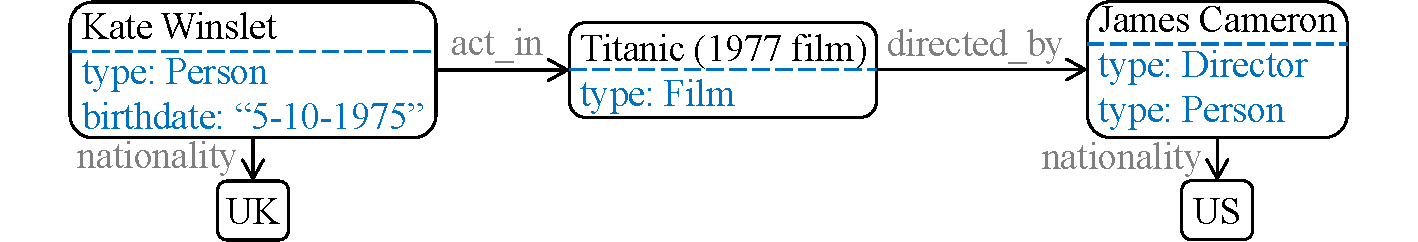
\includegraphics[width=\columnwidth]{figs/qpcsg.pdf}
\caption{A summary extracted from Figure~\ref{fig:example} exemplifying the two EDPs and the LP in Figure~\ref{fig:edp-lp}, and containing the query keywords \textit{Titanic} and \textit{US}.}
\label{fig:qpcsg}
\end{figure}

\subsubsection{Diameter-Bounded Max-Coverage Group Steiner Tree}
The standard GST problem requires the extracted tree to cover all the groups, but this is not always achievable in practice. For example, given a KG that is a disconnected graph, a tree that connects all the keywords in a query may not exist. Even for a connected graph, a large tree may have to be extracted to cover keywords that are distant from each other in the graph structure, against the goal of extracting a compact summary. To achieve a trade-off between query coverage and structural compactness, Cheng et al.~\shortcite{DBLP:conf/semweb/ChengLZL20} propose to allow relaxing a query by ignoring a minimum number of keywords to guarantee the compactness of the extracted summary.

As a generalization of this idea, Zhang et al.~\shortcite{DBLP:conf/www/ZhangW023} formulate a \emph{Diameter-bounded max-Coverage Group Steiner Tree} (DCGST) problem. Compared with a standard GST, DCGST has a bounded diameter and is required to cover not necessarily all but the most possible groups. For example, given a keyword query \textit{Titanic US talking} over Figure~\ref{fig:example} and a diameter bound of two hops, the summary extracted here has to ignore the keyword \textit{talking} but choose to be concisely focused on the connection between the other two keywords, as illustrated in Figure~\ref{fig:gst}. By contrast, the summary extracted by the aforementioned KeyKG approach is a standard GST consisting of a long and unfocused path, as shown in Figure~\ref{fig:non-dcgst}, although it covers all the three keywords. The DCGST problem is an emerging NP-hard optimization problem and is solved by PrunedCBA~\cite{DBLP:conf/www/ZhangW023}, an approximation algorithm performing pruned best-first search based on a novel hop-bounded index of precomputed distances.

\begin{figure}[h]
\centering
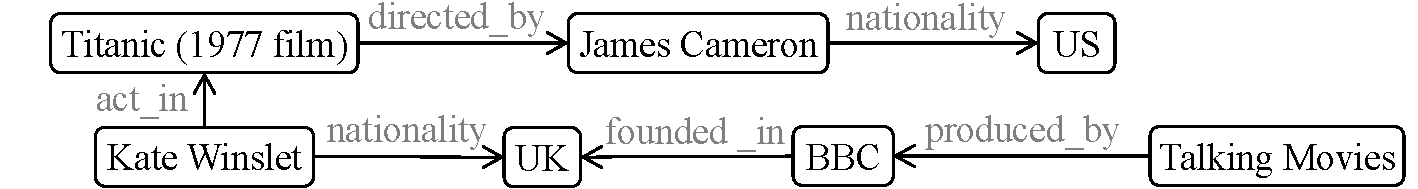
\includegraphics[width=\columnwidth]{figs/dcgst.pdf}
\caption{A summary extracted from Figure~\ref{fig:example} containing a long path that connects the query keywords \textit{Titanic}, \textit{US}, and \textit{talking}.}
\label{fig:non-dcgst}
\end{figure}

\subsubsection{Quadratic Group Steiner Tree}
Another extension of the GST formulation for query-biased KG summarization considers the semantic cohesiveness of the extracted tree~\cite{DBLP:conf/bigdataconf/ChengK17}. Recall that the standard minimum-weight GST problem optimizes the total weight of the extracted nodes or edges, where weights reflect (inverse) salience. However, a set of salient nodes or edges may not always comprise a meaningful connection as a whole. It can be a semantically disjointed tree that connects a set of salient but disparate entities. To improve semantic cohesiveness, Shi et al.~\shortcite{DBLP:conf/www/Shi0TKS21,DBLP:conf/ijcai/Shi0T0K21} incorporate the minimization of semantic distances between extracted entities into the objective function. They formulate a more generalized \emph{Quadratic Group Steiner Tree} (QGST) problem. Compared with a standard GST, QGST minimizes a linear combination of the sum of weights of its nodes and the sum of quadratic weights of its node pairs. Quadratic weight characterizes the semantic distance between a pair of entities, e.g., the angular distance between their embedding vectors. The extracted summary tends to include entities that are not only salient by themselves and matched with the query, but also semantically close to each other, hence forming a semantically cohesive whole. For example, given a keyword query \textit{Avatar DiCaprio}, the top tree in Figure~\ref{fig:qgst} contains salient entities like \texttt{US} but also disparate entities including a film, a director, a country, and an actor. By contrast, the entities in the bottom tree are a set of closely related films and actors, representing a more meaningful connection. To solve the QGST problem which is an NP-hard optimization problem, B$^3$F~\cite{DBLP:conf/ijcai/Shi0T0K21} is an exact algorithm that performs branch-and-bound best-first search. QO and EO~\cite{DBLP:conf/www/Shi0TKS21} are two approximation algorithms with the idea of finding and merging small-weight paths from a root node to all the groups.

\begin{figure}[h]
\centering
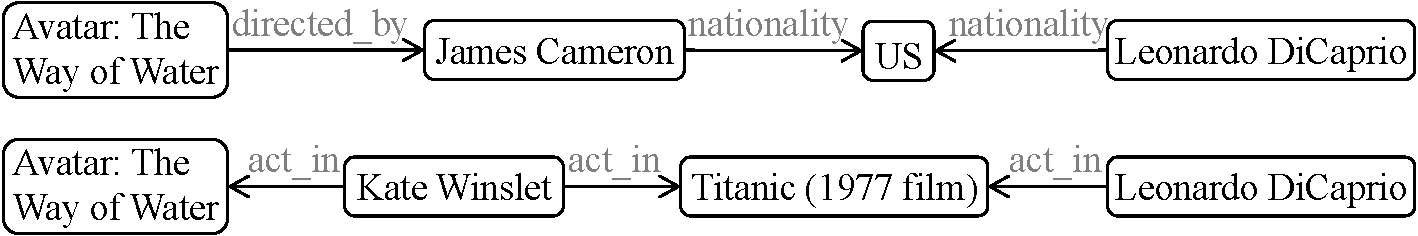
\includegraphics[width=\columnwidth]{figs/qgst.pdf}
\caption{Two summaries extracted from Figure~\ref{fig:example} containing the query keywords \textit{Avatar} and \textit{DiCaprio}.}
\label{fig:qgst}
\end{figure}

\paragraph{Remarks}
Compared with maximum coverage, GST-based formulations are expressive but hard to solve. Although KeyKG and PrunedCBA perform satisfyingly on large KGs with millions of nodes, they rely on a precomputed distance index which needs to be rebuilt when the KG evolves. For the QGST problem, no algorithm so far could respond to a query over a million-scale KG in real time. All these limitations should be taken into account when choosing the formulation.

\subsection{Personalized Summarization}

Besides keyword queries, users' interests can be explicitly expressed or implicitly discovered in various manners. Serving the user with a personalized summary extracted from a large KG provides cost-effectiveness in KG reuse~\cite{DBLP:conf/icdm/SafaviBFMMK19,DBLP:conf/esws/VassiliouAPK23}. Existing methods in this category tailor KGs to a user's needs in different forms: a single entity of interest, a class representing a domain or a set of entities specified by the user, or the user's own query history.

\subsubsection{Single Entity}
The iSummary approach~\cite{DBLP:conf/esws/VassiliouAPK23} allows the user to specify an entity of interest in the KG as a \emph{seed entity}, such as \texttt{James Cameron}, and it extracts a summary that compactly describes this entity as well as a set of its closely related entities. Specifically, each entity in the KG is assigned a weight. An entity with a higher frequency of co-occurrence with the seed entity in the query log has a higher weight. This frequency is believed to reflect the relatedness between entities. From the resulting node-weighted graph, a maximum-weight tree that connects the seed entity with its most related entities is extracted. This computational problem resembles the minimum-weight \emph{Steiner Tree} problem and is NP-hard. It is solved by an approximation algorithm that extracts shortest paths to connect the seed entity with its most related entities.

\subsubsection{Multiple Entities (in a Domain)}
A user may also want to extract a domain-specific summary from a large KG. A domain of interest can be represented by a set of \emph{in-domain entities}, e.g., all the entities having a particular type such as \texttt{Film} in Figure~\ref{fig:example}. To fulfill this need, Lalithsena et al.~\shortcite{DBLP:conf/bigdataconf/LalithsenaKS16} traverse the KG starting from in-domain entities to extract domain-specific edges. Their primary focus is to determine the domain specificity score of each relation type, and they present two measures. The first measure utilizes the strength of association among the types of relations and intermediate entities derived from instance-level frequencies. The second and more effective measure relies on the domain specificity of intermediate relations and adopts Pointwise Mutual Information for measuring association.

In a follow-up work, Lalithsena et al.~\shortcite{DBLP:conf/bigdataconf/LalithsenaPKS17} further employ the Wikipedia categories of each entity and restrict graph traverse to the entities in the top-ranked domain-specific categories. To determine the domain specificity score of a category, they collect evidences from the types of the entities in the category, its lexical label, and its structural abstractness characterized by its outdegree in the category hierarchy. Evidences are aggregated for ranking categories using Probabilistic Soft Logic, a statistical relational learning framework.

Instead of graph traversal, Jiang et al.~\shortcite{DBLP:conf/adma/JiangZGGWZ12} firstly mine the frequent subgraph patterns in a KG, and extract their instance subgraphs that contain user-specified entities. These subgraphs are merged by intersection or union into a single graph, where each edge is weighted based on a combination of the frequencies of its constituent entities and relation type. Finally, a minimum-weight Steiner Tree that connects all the user-specified entities is extracted from this graph as a summary of the semantic associations among those entities.

Here we would like to distinguish the approaches in this category from the research on \emph{relationship search}~\cite{DBLP:journals/sigweb/000120}, i.e.,~searching and ranking subgraphs that connect a given set of input entities~\cite{DBLP:journals/tkde/ChengSQ17}.
% DBLP:journals/tkde/ChengLQ21
Their main difference is that the approaches here extract and summarize all the subgraphs relevant to the input entities, whereas relationship search is only focused on finding a few top-ranked subgraphs to be presented as search results.

\subsubsection{Query History}
When a user's personal query history is available, the GLIMPSE approach~\cite{DBLP:conf/icdm/SafaviBFMMK19} extracts a personalized summary from a KG containing only a subgraph most relevant to the user's interest reflected in past queries. To this end, entities and relations are scored by a probabilistic framework estimated from their frequencies observed in the user's query history. The extraction of a size-bounded optimum subgraph is formulated as an optimization problem with a submodular objective function, hence featuring a greedy constant-factor approximation algorithm.

\paragraph{Remarks}
Despite the diverse forms of expressing a user's needs, it is possible to convert them into each other to be handled in a consistent manner. For example, from a user's query history, a set of frequent entities can be mined, which, in turn, can be processed separately as single entities.